
\documentclass[11pt,a4paper]{article}
\usepackage[utf8]{inputenc}
\usepackage[T1]{fontenc}
\usepackage[spanish,es-nodecimaldot]{babel}
\usepackage[a4paper,left=1.7cm,right=1.7cm,top=20mm,bottom=20mm]{geometry}
\usepackage{amsmath,amssymb,amsfonts,mathtools,bm}
\usepackage{braket}
\usepackage{graphicx}
\usepackage{float}
\usepackage{booktabs}
\usepackage{enumitem}
\usepackage{xcolor}
\usepackage{lmodern,microtype}
\usepackage{fancyhdr}
\usepackage{titlesec}
\usepackage[colorlinks=true,linkcolor=black,urlcolor=black,citecolor=black]{hyperref}
\numberwithin{equation}{section}
\renewcommand{\boxed}[1]{#1}
\setlength{\parindent}{0pt}
\setlength{\parskip}{5pt}
\newcommand{\dd}{\,\mathrm d}
\newcommand{\ii}{\mathrm i}
\newcommand{\e}{\mathrm e}
\newcommand{\hb}{\hbar}
\newcommand{\R}{\mathbb R}
\newcommand{\C}{\mathbb C}
\newcommand{\id}{\mathbb I}

\pagestyle{fancy}
\setlength{\headheight}{14pt}
\fancyhf{}
\fancyhead[L]{\textit{Tarea 15}}
\fancyhead[R]{Mecánica Cuántica I}
\begin{document}
\begin{titlepage}
\centering
\vspace*{1.8cm}

\includegraphics[width=.22\textwidth]{UdeC_escudo.png}
\vspace{1.1cm}
{\Huge\bfseries Tarea 15\par}
\vspace{.4cm}
{\Huge\bfseries Mecánica Cuántica I\par}
\vspace{1.5cm}
{\Large José Ignacio Rosas Sepúlveda\par}
\vspace{.8cm}
{\Large Solución\par}
\vfill
\thispagestyle{empty}
\end{titlepage}
\tableofcontents
\newpage
\section*{Enunciado}
\addcontentsline{toc}{section}{Enunciado}
\begin{enumerate}[label=\arabic*.]
\item Como $a$ no es hermítico, sus valores propios $\alpha$ pueden ser complejos y sus estados propios $\ket\alpha$ no son ortogonales. Demuestre que
\begin{equation}
\braket{\alpha|\beta}=\exp\left[-\frac{|\alpha|^2+|\beta|^2}{2}+\alpha^*\beta\right].
\end{equation}
\item Grafique $|\braket{\alpha|1+i}|^2$ como función de $\operatorname{Re}\alpha$ e $\operatorname{Im}\alpha$.
\item Demuestre que $\ket\alpha\to\ket0$ cuando $\alpha\to0$.
\item Un oscilador armónico está inicialmente en la superposición impar
\begin{equation}
\ket{\psi(0)}=N(\ket\alpha-\ket{-\alpha}),\qquad \alpha\in\mathbb R.
\end{equation}
\begin{enumerate}[label=\alph*)]
\item Encuentre $N$.
\item Encuentre el límite $\alpha\to0$.
\item Encuentre $\ket{\psi(t)}$.
\item Calcule la probabilidad de encontrar el sistema en $\ket\alpha$.
\item Calcule la probabilidad de encontrar el sistema en $\ket{-\alpha}$.
\item Calcule la probabilidad de retorno al estado inicial.
\item Encuentre la distribución de probabilidad del número de fotones y grafíquela para $\alpha=\sqrt3$ y $\alpha=3$.
\end{enumerate}
\end{enumerate}


\section{Problema 1}
Usamos
\begin{equation}
\ket\alpha=\e^{-|\alpha|^2/2}\sum_{n=0}^{\infty}\frac{\alpha^n}{\sqrt{n!}}\ket n.
\end{equation}
Entonces
\begin{align}
\braket{\alpha|\beta}
&=\e^{-(|\alpha|^2+|\beta|^2)/2}
\sum_{n=0}^{\infty}\frac{(\alpha^*\beta)^n}{n!}\\
&=\boxed{\exp\left[-\frac{|\alpha|^2+|\beta|^2}{2}+\alpha^*\beta\right]}.
\end{align}
Su módulo es
\begin{equation}
\boxed{|\braket{\alpha|\beta}|^2=\e^{-|\alpha-\beta|^2}.}
\end{equation}
La no ortogonalidad es una propiedad esencial de los estados coherentes.

Para $\beta=1+\ii$,
\begin{equation}
|\braket{\alpha|1+\ii}|^2=
\exp[-(\operatorname{Re}\alpha-1)^2-(\operatorname{Im}\alpha-1)^2].
\end{equation}
\begin{figure}[H]\centering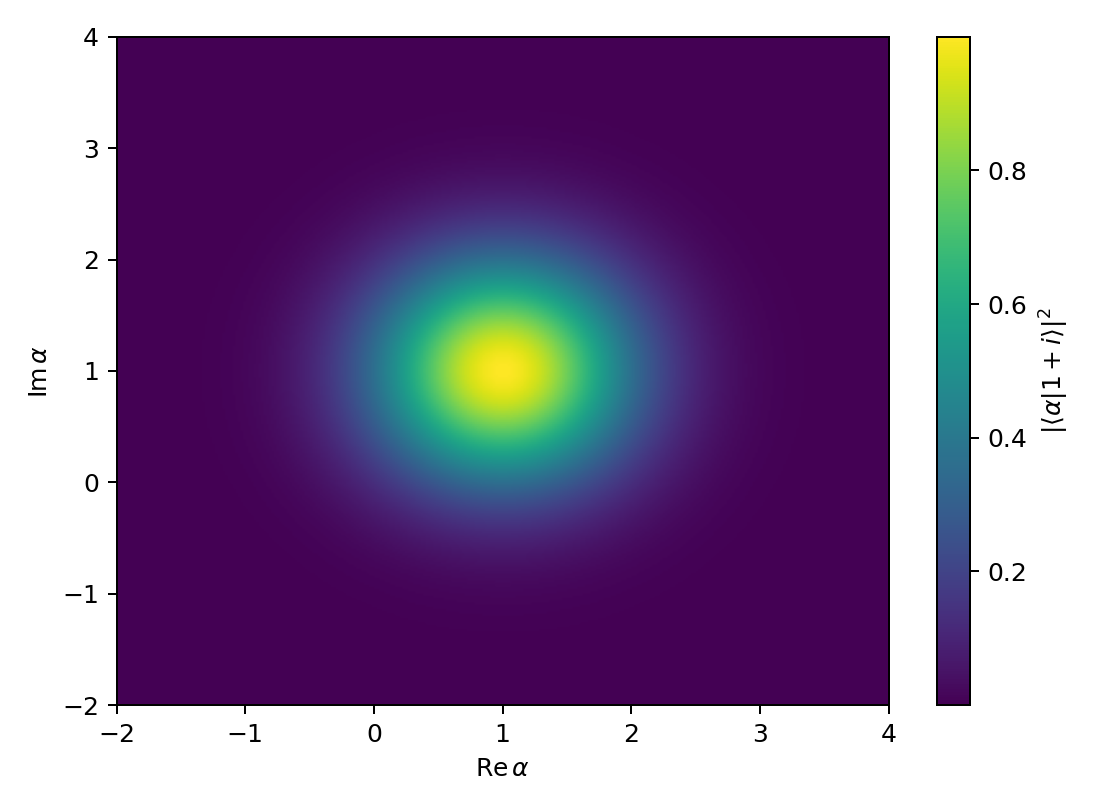
\includegraphics[width=.66\textwidth]{figures/overlap_coherentes.png}\caption{Solapamiento con el estado $\ket{1+\ii}$.}\end{figure}

\section{Problema 2}
De la expansión en estados número,
\begin{equation}
\ket\alpha=\e^{-|\alpha|^2/2}
\left(\ket0+\alpha\ket1+\frac{\alpha^2}{\sqrt2}\ket2+\cdots\right),
\end{equation}
por lo que
\begin{equation}
\boxed{\lim_{\alpha\to0}\ket\alpha=\ket0.}
\end{equation}

\section{Problema 3}
Para $\alpha\in\R$,
\begin{equation}
\ket{\psi(0)}=N(\ket\alpha-\ket{-\alpha}).
\end{equation}
Como $\braket{\alpha|-\alpha}=\e^{-2\alpha^2}$,
\begin{equation}
\boxed{N=\frac{1}{\sqrt{2(1-\e^{-2\alpha^2})}}.}
\end{equation}
En el límite $\alpha\to0^+$,
\begin{equation}
\ket\alpha-\ket{-\alpha}=2\alpha\ket1+O(\alpha^3),
\end{equation}
y $N\sim1/(2\alpha)$. Por tanto
\begin{equation}
\boxed{\lim_{\alpha\to0^+}\ket{\psi(0)}=\ket1.}
\end{equation}

Para el oscilador armónico,
\begin{equation}
U(t)\ket\alpha=\e^{-\ii\omega t/2}\ket{\alpha\e^{-\ii\omega t}}.
\end{equation}
Definiendo $\alpha_t=\alpha\e^{-\ii\omega t}$,
\begin{equation}
\boxed{\ket{\psi(t)}=N\e^{-\ii\omega t/2}(\ket{\alpha_t}-\ket{-\alpha_t}).}
\end{equation}
Las probabilidades de proyectar sobre $\ket{\pm\alpha}$ son iguales:
\begin{equation}
\boxed{P_{+\alpha}(t)=P_{-\alpha}(t)
=4N^2\e^{-2\alpha^2}\left|\sinh(\alpha^2\e^{-\ii\omega t})\right|^2.}
\end{equation}
La probabilidad de retorno al estado inicial es
\begin{equation}
\boxed{P_{\psi(0)}(t)=
16N^4\e^{-2\alpha^2}\left|\sinh(\alpha^2\e^{-\ii\omega t})\right|^2.}
\end{equation}

La distribución de fotones contiene sólo números impares:
\begin{equation}
\boxed{P_n=\begin{cases}
4N^2\e^{-\alpha^2}\dfrac{\alpha^{2n}}{n!},&n\ \text{impar},\\[5pt]
0,&n\ \text{par}.
\end{cases}}
\end{equation}
\begin{figure}[H]\centering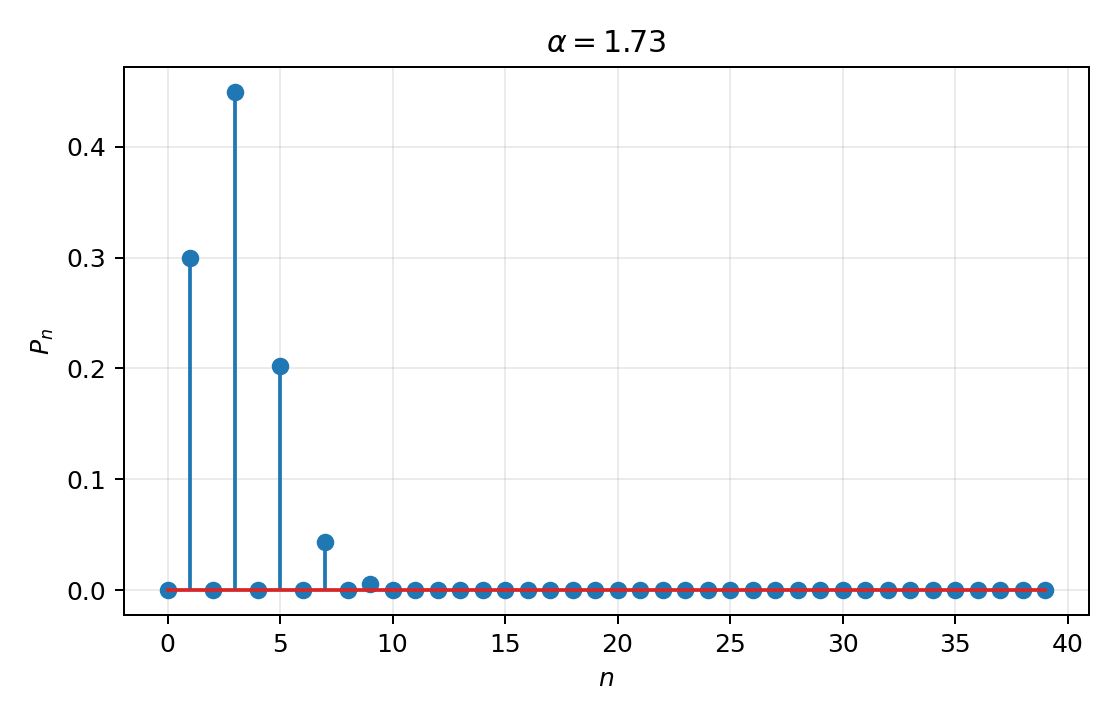
\includegraphics[width=.65\textwidth]{figures/fotones_alpha_sqrt3.png}\caption{Distribución para $\alpha=\sqrt3$.}\end{figure}
\begin{figure}[H]\centering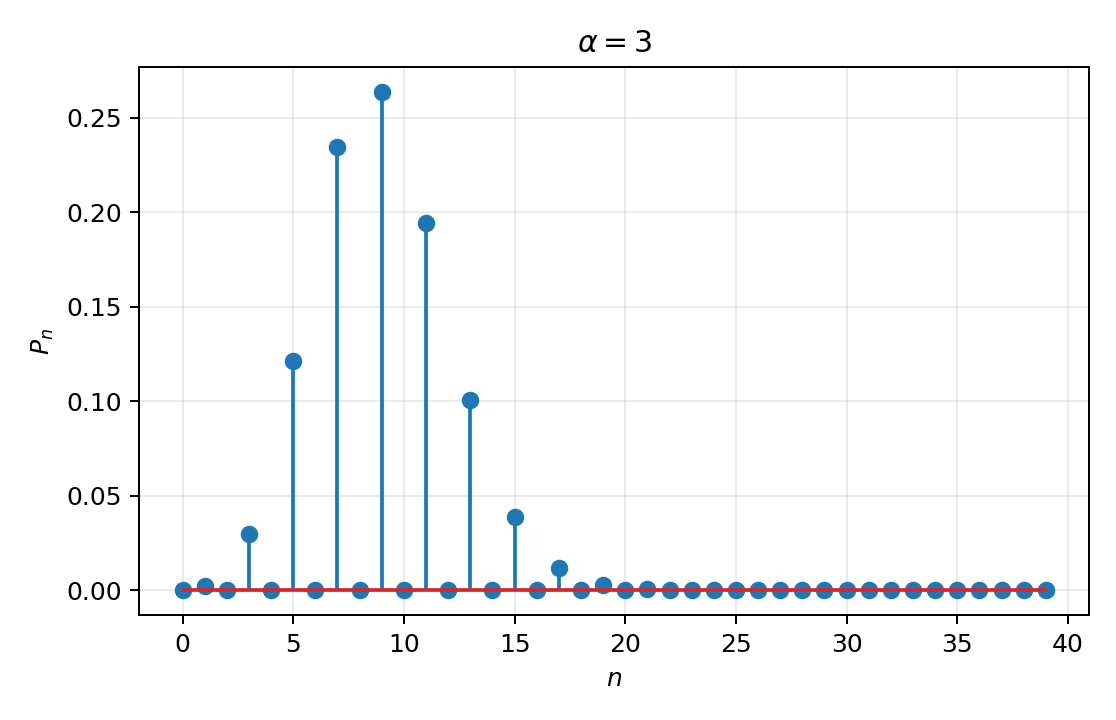
\includegraphics[width=.65\textwidth]{figures/fotones_alpha_3.png}\caption{Distribución para $\alpha=3$.}\end{figure}


\end{document}
